\chapter{Introduction and Motivation}
\label{ch:intro}


\section{Motivation}
\label{sec:motivation}


Since the discovery (and further confirmation) of the greenhouse effect in the years from 1824 to 1900 \cite{fourier1824remarques, foote1856circumstances} mankind has come a long way in combating the consequences of the increased concentration of greenhouse gases in the Earth's atmosphere. 
% In 1972 \citeauthor{sawyer1972man} summarized the knowledge and predicted quite accurately the warming at the end of the century \cite{sawyer1972man}.
Especially in the last decades, the climate crisis has gained more and more attention, leading to the creation of several international organizations and institutions (e.g., the \ac{ipcc} in 1988).
In 2019, more than 11,000 scientists from around the world issued a statement \cite{ripple_world_2019} calling on governments around the world to take action.




\begin{figure}[hbt]
  \begin{center}
    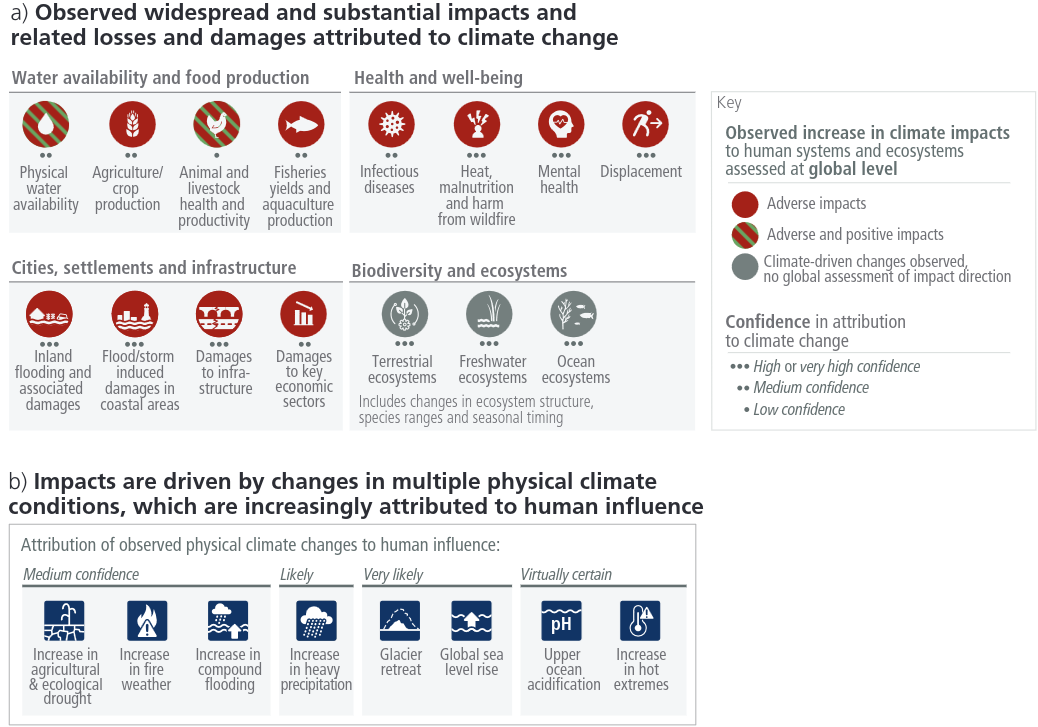
\includegraphics[width=0.85\textwidth]{figures/ipcc_6th_report_impacts_climate_change.png}
  \end{center}
  \caption{Impact of Climate Change for Humans, taken from the 6th IPCC report for policymakers \cite{lee2024climate}}
  \label{fig:impacts_climate_change}
\end{figure}



The consequences for the environment and humans are prevalent and are, in part, already visible today. 
Figure \ref{fig:impacts_climate_change} shows likely consequences for humans from the latest IPCC report for policymakers \cite{lee2024climate}: Flooding, malnutrition, displacement, and damages to ecosystems can be attributed with high confidence to climate change. 

Atmospheric moisture and precipitation are main part of the water cycle and provide large parts of the water consumed by plants, crops, animals and humans. 
The variability of precipitation, and its main source, atmospheric moisture transport are drivers of floods and droughts, as well as they play a vital role for humans and ecological systems.  
The variability in these processes is significantly influenced by dominant oscillation systems, such as the \ac{nao} in Europe and the \ac{enso} in South America.
Recent research shows that big circulation systems like the \ac{nao} \cite{vietinghoff_visual_2021} change as well in the face of climate change, depending on its intensity.  
This thesis aims to investigate the implications of these changes specifically in the context of moisture transport.
Moisture transport, a critical component of the atmospheric system, presents significant challenges for analysis due to its inherently oscillating nature.
To address the complexity of moisture transport, the Thesis tries to tackle this issue by employing pattern analysis to track the structural changes of moisture and a sliding window approach (motivated by the research of \citeauthor{vietinghoff_visual_2021}) to identify and understand structural changes in moisture transport mechanisms in Europe and the Northern Atlantic. 
Furthermore, reducing the turbulent flow of moisture to its dominant patterns helps to address one of the major challenges in modern climate science: the uncertainty associated with multiple simulation results and the reduction of the immense volume of data.\todo{Gerne bisschen ausführlicher und motivierender, tatsächliche Arbeit eher auf einem high level} 
% By analyzing and interpreting the variability across different simulation members, this study contributes to a more robust understanding of moisture transport and its future evolution in Europe. 
% The mid and long-term consequences are manyfold and go far beyond the general rising of the worlds' average temperature (see Figure \ref{fig:impacts_climate_change}), e.g., shifts in circulation systems like the North Atlantic Oscillation (\ac{nao}) \cite{vietinghoff_visual_2021}, which in turn also have varying consequences. 

% Although the water vapor in the air accounts for only 0.001 \% of the water on the earth, it is the most active part of that cycle \cite{zou_investigating_2020}. 
% Also, research shows that the precipitation on land does not match the evaporation, meaning the water was transported (from the oceans) to land, providing water for the ecosystems there.  \todo{CITE!!! Where the fuck did I read this?}
% Analyzing the structural change of this moisture transport, its causes and its consequences could help understanding more about the future of climate change. 
%
% Motivated by the research of \citeauthor{vietinghoff_visual_2021}, this thesis aims to evaluate similarly the systemic changes of moisture transport and precipitation patterns in Europe and the northern Atlantic.
%
% Climate change is fundamentally altering the oscillation systems responsible for variability in atmospheric conditions. 
%


\section{Climate and Climate Research}
\label{sec:climate}

% This section should give an introduction to the current state of climate research. 
% Therefor it should explain what the current way of future climate predictions is (Coupled Models), how they work, and 
% It should explain some part of the politics, who is involed in what and what the backroud of the most important projects (\ac{cmip}, ScenarioMIP \dots). 
% It should be explained that the data used is the one that the highest council of fighting climate change uses for its report. 


\subsection{Quick Overview over Climate Systems and Climate Change}


While weather is the momentary state of the atmosphere at a time, climate is the average of weather patterns over a larger period of time, usually 30 years or more \cite{noaa_whats_nodate}. 
So the term climate change does not refer to any unexpected weather changes, but to the structural changes of said patterns over a large period of time (e.g., the warming of the global average temperature). 
Earth's climate system can be seen as complex interactions of its major components: atmosphere, hydrosphere, cryosphere, lithosphere, and biosphere \cite{vietinghoffdiss, intergovernmental_panel_on_climate_change_ipcc_climate_2023}. 
Changes in this system can have (roughly) two reasons: 
Either redistributions of energy, presenting themselves as internal oscillations, which can happen on arbitrary large scales\footnote{See the discussion on the change of the Atlantic meridional overturning circulation in the work of \citeauthorwork{lobelle_detectability_2020}, which could be a multiple-decades-spanning oscillation} or in the form of external forcings \cite{vietinghoffdiss}. 
External forcings influence the system from outside sources, such as volcanic activity, variations in solar radiation, and, importantly, the emission of \ac{ghg}. 

\begin{figure}[htb]
  \begin{center}
    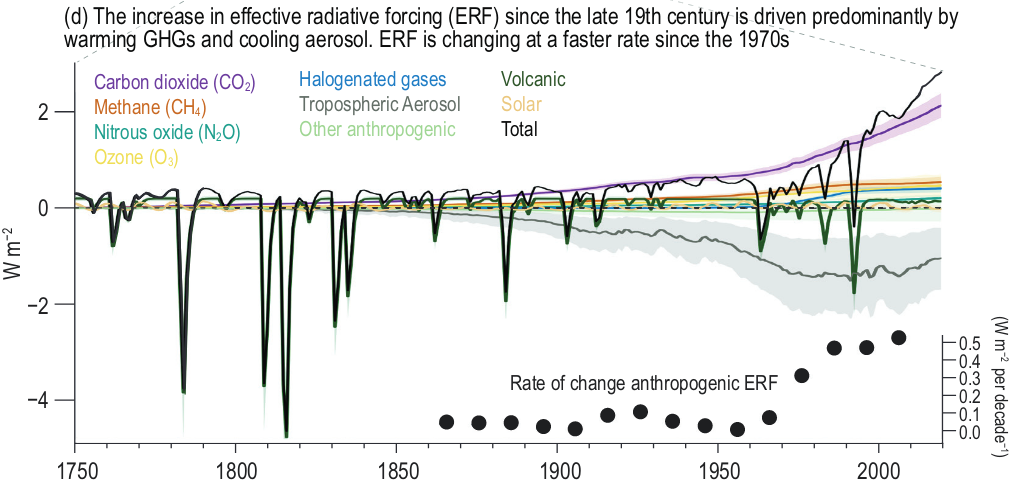
\includegraphics[width=0.95\textwidth]{figures/ERF_change_with_forcings.png}
  \end{center}
  \caption{The evolution of the effective radiative forcing and contributing components, taken from \cite{intergovernmental_panel_on_climate_change_ipcc_climate_2023}. The black line indicates the total \ac{erf}, while the contributions of different forcings are colored. Black dots at the bottom indicate the rate of anthropogenic \ac{erf} change.}
  \label{fig:erf-with-forcings}
\end{figure}

Figure \ref{fig:erf-with-forcings} shows an example of an effect of such external forcings: It displays the change in \ac{erf} and its contributing components over the last 2.5 centuries. 
\ac{erf} (in $Wm^{-2}$) is a way of measuring how much energy from the sun is \enquote{trapped} instead of reflected back to space (greenhouse effect). 
A positive value means warming, while a negative value is associated with cooling. 
As illustrated in  Figure \ref{fig:erf-with-forcings}, there was no significant change in the natural forcings (volcanic or solar radiation), the main drivers of change in \ac{erf} are clearly the man-made \acp{ghg} and cooling aerosols. \cite{intergovernmental_panel_on_climate_change_ipcc_climate_2023}

Regarding the internal variations: Most of it is part of spatio-temporal, cyclic pattern. Especially the interaction of the atmosphere with the hydrosphere (i.e. all liquid forms of water on earth) are responsible for large parts of climate's internal variations on decadal and interannual time frames \cite{vietinghoffdiss}. 
Prominent examples for such oscillations are the \ac{enso} or the \ac{nao}, the latter one being especially relevant for this thesis. 


\subsection{The North Atlantic Oscillation}
\label{sec:nao}


The aforementioned \ac{nao} is \enquote{one of the most recurrent and prominent patterns of atmospheric circulation variability} \cite{hurrell_overview_2003}. 
It is also one of the oldest known weather patterns, since descriptions of Scandinavians exist from centuries back. 
It dictates the climate variability for a large area: From the East Coast of the USA to Siberia and from the Arctic to the subtropical Atlantic.
Especially in the boreal winter (usually from December to February), the variations of the \ac{nao} influences a wide range of variability areas: From the mean wind speed and direction to the heat and moisture transport as well as the intensity and amount of storms and their path. \cite{hurrell_overview_2003}

\begin{figure}[htb]
  \begin{center}
    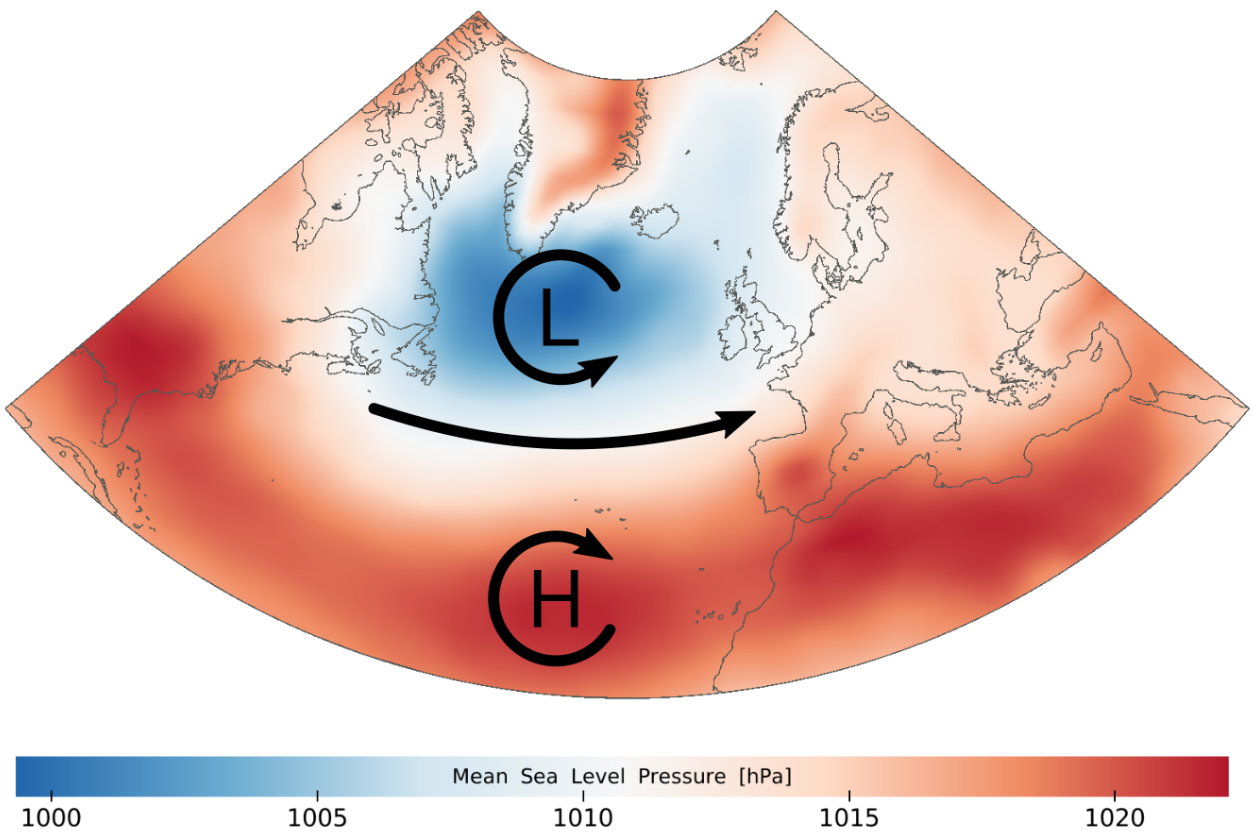
\includegraphics[width=0.75\textwidth]{figures/nao_pattern_diss.png}
  \end{center}
  \caption{Characteristic mean SLP field of a boreal winter season, taken from \cite{vietinghoffdiss}. It shows a high (H)/low (L) pressure pattern, directing air from the Atlantic westwards towards Europe. }
  \label{fig:naopattern}
\end{figure}


The \ac{nao} is a redistribution of atmospheric mass from the Arctic to the subtropical Atlantic, producing the aforementioned effects while swinging from one phase to another. 
Its basis is a characteristic dipole in the Sea Level Pressure Field (SLP) of the Atlantic (see Figure \ref{fig:naopattern}).
Due to the Coriolis Force, air flows clockwise around high pressure and counterclockwise around low pressure in the Northern Hemisphere, leading to the transport of the maritime air from the Atlantic towards Europe (see Figure~\ref{fig:naopattern}) \cite{hurrell_overview_2003, vietinghoffdiss}. 
Depending on the pressure differences, the effect varies: high pressure differences lead to higher transport of mild, humid air to Europe, which in turn results in milder European winters. In contrast, a low difference leads to a less pronounced effect and therefor to colder winters. 
These pressure differences vary on an interannual scale, and this effect is called the North Atlantic Oscillation. 
Figure~\ref{fig:naoindex_comparison} illustrates the \ac{nao} index, which is based on measurements of weather stations in Iceland and the Azores (top row), and which represents the conventional methodology for defining the \ac{nao}. 
Another method is by computing the first/dominant Empirical Orthogonal Function (the pattern analysis technique employed in this Thesis, see Section~\ref{sec:eof}) of the sea level pressure field in wintry North Atlantic/Europe, the temporal coefficients (or Principal Components) (middle row) are a good estimate of the measured Index. 

\begin{figure}[htb]
  \begin{center}
    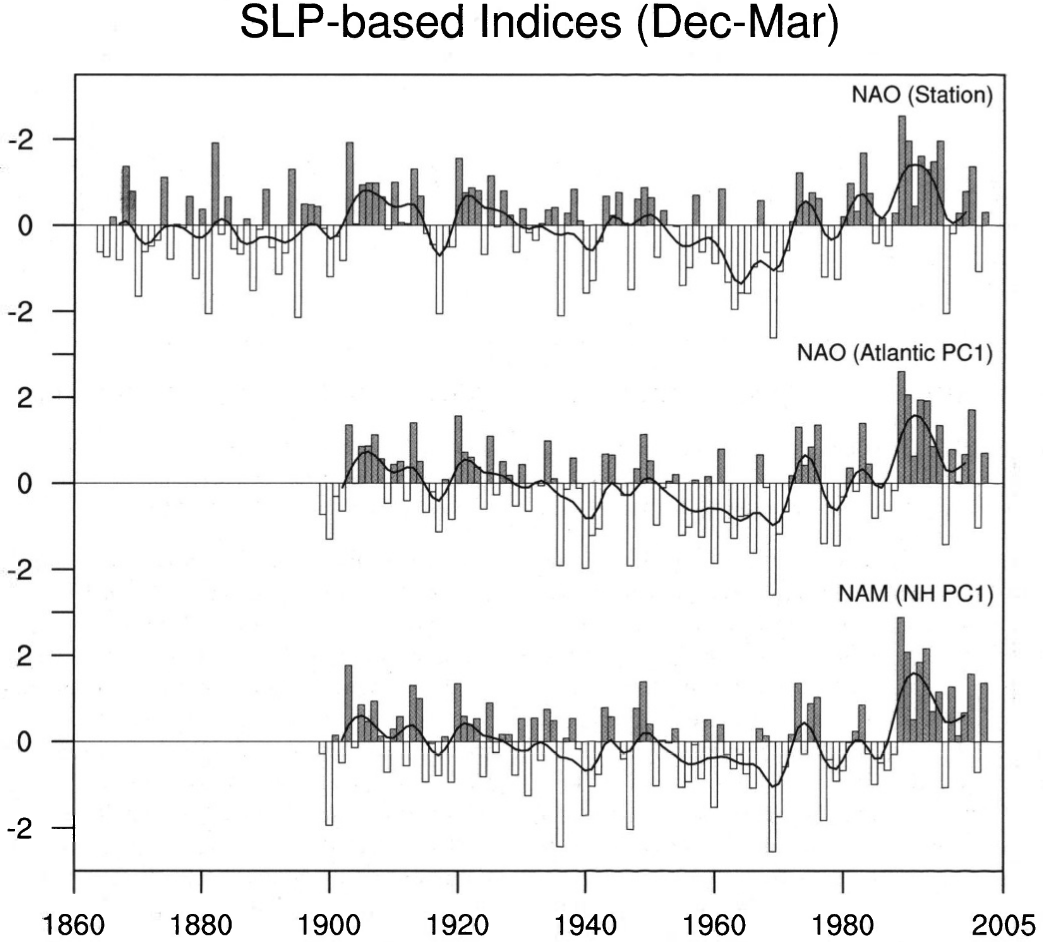
\includegraphics[width=0.75\textwidth]{figures/hurrel_nao_index_comparison.png}
  \end{center}
  \caption{Comparison of the \ac{nao} index from \cite{hurrell_overview_2003}: The top panel are differences of SLP from weather stations in Portugal and Iceland, the middle panel is the first principal component of corresponding to the first \ac{eof} of the northern Atlantic SLP field, and the bottom panel is the same as the middle panel but for the whole Northern Hemisphere. See \cite{hurrell_overview_2003} for a more detailed description}
  \label{fig:naoindex_comparison}
\end{figure}

A large fraction of the recent warming in Europe can be linked to the behavior of the \ac{nao} in the last decades: it shifted from large amplitude anomalies in the negative to similar anomalies in the opposite direction in the later years. 
Therefor, \citeauthor{hurrell_overview_2003} points out the need to study the relationship of anthropogenic climate change and the \ac{nao}. 
Following the argumentation of \citeauthorwork{hurrell_overview_2003}, the motivation of this thesis by \citeauthorwork{vietinghoff_visual_2021} tried to track the shift of the centers of the dipoles in different climate scenarios.   

\begin{figure}
  \begin{center}
    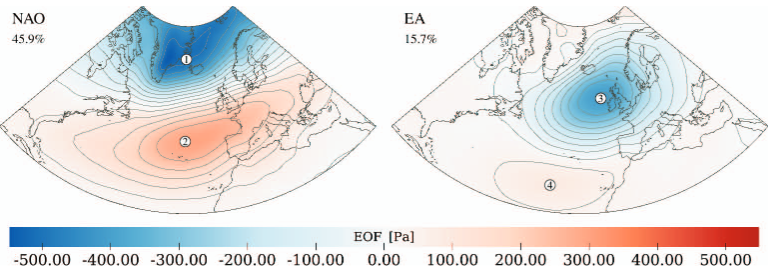
\includegraphics[width=0.95\textwidth]{figures/nao_eap.png}
  \end{center}
  \caption{The most prominent modes of internal atmospheric variability in Europe/the Atlantic: The North Atlantic Oscillation (\ac{nao}) and East Atlantic Pattern (EAP) (taken from \cite{vietinghoff_extension_2021})}\label{fig:nao eap}
\end{figure}


Also worth mentioning is the East Atlantic Pattern (EAP, see Figure~\ref{fig:nao eap}), the second most prominent mode of internal atmospheric variability.
It is defined as the second Principal Component (\ac{eof}) of \ac{psl} in the Atlantic.  
It is characterized by a large Sea Level Pressure Anomaly in the west of the British Islands and less pronounced  anomalies in the subtropical Atlantic and Eastern Europe. 
Similar to the \ac{nao}, it is prominent throughout the winter and influences precipitation and temperature throughout Europe. \cite{comas-bru_effect_2016, song_east_2019}

\subsection{Climate Research: The IPCC and the \ac{cmip}}
\label{sec:climate research}


The rationale behind the UN General Assembly's endorsement of the \ac{ipcc} in 1988 was to facilitate the preparation of comprehensive reviews and reports concerning the current state of scientific knowledge and research. 
Subsequently, six assessment cycles have been conducted, resulting in the publication of six reports that synthesize the findings of the scientific community. 
Figure \ref{fig:impacts_climate_change}, taken from the most recent report for policymakers \cite{lee2024climate}, illustrates the potential impacts of climate change on humans.

The primary source for these figures in the reports is the so-called \acp{gcm}, which attempt to model the state and evolution of specific fields of Earth data.
These models are composed of multiple components, each representing a significant aspect of the Earth's intricate climate system, including the atmosphere and hydrosphere. 
Additionally, they facilitate the examination of the dynamic interactions between these components \cite{vietinghoffdiss}.  
In the mid-1990s, the \ac{cmip} was established with the objective of enhancing the consistency and comparability of \ac{gcm} results. 
\ac{cmip} provides the outer structure for the production of simulations, the type of simulation (e.g., preindustrial control simulations, future scenarios, etc.), the generation of fields, the provision of resolutions, and the serialization of results.
Subsequently, the results of \ac{cmip} have assumed an increasingly prominent role in \ac{ipcc} reports \cite{touzepeiffer_coupled_2020}, to the extent that they are now regarded as a foundational element of climate science \cite{eyring_overview_2016}. 
The \ac{cmip} is currently in its sixth phase, corresponding to the recently published sixth Assessment Report of the \ac{ipcc} \cite{lee2024climate}. 
The sixth phase describes an inner core (DECK\footnote{Diagnostic, Evaluation and Characterization of Klima. This is a set of baseline simulations which should be included in every coming CMIP iteration. An example of such an experiment is a preindustrial control simulation.} + historical simulations), which is a prerequisite for participation in \ac{cmip}. It also encompasses some endorsed \acp{mip}, which are optional. Examples of these include ScenarioMIP (future scenario simulations), HighResMIP (for exploring models with higher resolutions), and GeoMIP (exploring the effects of geoengineering). \cite{eyring_overview_2016}

The simulations are usually set up as so-called ensemble simulations. 
This means they consist of different members, which are one realization or run of a simulation. 
The members use the same forcings, but different starting conditions and are independent of each other. 
By using multiple simulations it is possible to separate the internal variability from the responses to the external forcing, enabling researchers to better quantify the consequences of climate change. 
Additionally, it makes the research of extreme weather phenomena (e.g., droughts, floods etc.) more robust in spite of their rare occurrences \cite{maher_large_2021}.
% This results in the challenge of working with more than one field (see Section~\ref{sec:uncertainfields}) and visualizing the variability introduced by multiple members. 
However, this approach also presents a challenge in terms of visualization, as it requires displaying multiple variants of the same data simultaneously, which can be difficult to do effectively.
This issue was also identified as a significant research problem in the field of scientific visualization \cite{johnson_top_2004}. 


\section{Research Questions and Thesis Structure}
\label{sec:research_questions}

Following up the previous sections, the research question for this thesis is: 

\begin{center}
  \larger{\enquote{How do the Patterns of Moisture Transport and precipitation change in the face of different climate scenarios in the North-East Atlantic?}}
\end{center}

The patterns are needed to reduce the sheer amount of data and to make it possible to compare different climate scenarios across multiple members of the simulation ensemble beyond simple statistics.
With this goal the broad research question can be broken down into smaller milestones: 

\subsubsection{M1: Generate the patterns of moisture transport and other variables}

The moisture transport needs to be somehow quantified, and this quantification needs to be calculated based on the data available in the chosen dataset (Chapter~\ref{ch:dataset}). 
Furthermore, a similar sliding window approach as in \cite{vietinghoff_visual_2021} needs to be implemented to study the evolution of the patterns.
The challenge is hereby the large size of datasets due to multiple members, scenarios, and the combination of a large time scope and temporal resolution. 
% THos include the patterns of the quantified moisture transport, preciptation and surface level pressure (\ac{psl}), which can be used as the \ac{nao} index (see Figure~\ref{fig:naoindex_comparison}) and can be used t

\subsubsection{M2: Study the relationships with other variables and patterns}

To get a grasp of the meaning of the moisture transport, the connection or relation to other variables (see Section~\ref{sec:Position of this Thesis}) and patterns needs to be explored. 
% This can be achieved by analyzing the connection of moisture transport patterns with precipitation or the activity of sea level pressure patterns. 
The first connection should be to the \ac{nao}, or generally, patterns of surface pressure levels (such as the East Atlantic Pattern, the second most significant mode of \ac{psl} \ac{eof}). 
The second connection should be precipitation (patterns), as one of the most important consequences of transported moisture and the great influence on ecological and economic systems. 


\subsubsection{M3: Visualize the results}

The patterns, its components and their relationships with each other and variables need to visualized so that they can properly be interpreted. 
It is important here to visualize the variability introduced by uncertain fields (introduced by multiple members of the ensemble simulation).  
This includes selecting a feature in the results that can be used to analyze this variability and its change over time. 
E.g, one interesting thing to find if moisture transport experiences a similar shift to the north similar to the results of \citeauthorwork{vietinghoff_visual_2021}.

The goal of this thesis is not to interpret the results, but rather providing ideas, algorithms and visualizations for climate scientists to interpret the results of changing moisture transport \ac{eof} patterns. 




\vspace{.3cm}
The remaining thesis is structured as follows: Chapter \ref{ch:basics} introduces the theoretical background on fields and pattern analysis. 
The following Chapter \ref{ch:dataset} provides a detailed overview about the used \ac{cmip}6 based dataset. 
Chapter \ref{ch:related_work} provides an overview of related work, the motivation for this thesis and the position of this thesis in the academic context. 
While the results are discussed and presented in Chapter \ref{ch:results}, Chapter \ref{ch:methodology} gives a detailed description how these results came about. 
The thesis is concluded with Chapter \ref{ch:conclusions} where an outlook for potential future research is presented as well. 

